
\documentclass[a4paper]{article}

\usepackage[english]{babel}
\usepackage[utf8]{inputenc}
\usepackage{graphicx}
\usepackage{float}
\usepackage{amsmath}
\usepackage{listings}
\lst{language=Java, breaklines=true}

\author{Tamlin Love}

\date{\today}

\begin{document}
\begin{titlepage}
	\centering
	

\includegraphics[scale=0.6]{index.png}
	\vspace{0.5cm}
	
\newcommand{\HRule}{\rule{\linewidth}{0.5mm}} 

{\scshape\Large University of Witwatersrand\par}
{\scshape\Large Johannesburg, South Africa\par}
	\vspace{1cm}
	{\huge\bfseries Advanced Analysis of Algorithms\par}
	\vspace{1cm}
	{\Large\itshape Tamlin Love\par}
	\vspace{0.5cm}
	{\Large\itshape 1438243\par}
	\vfill
	
\HRule \\[0.4cm]
{ \huge \bfseries Lab Exam}\\[0.4cm] 
\HRule \\[1.5cm]

	{\large Semester 2, 2018\par}

\end{titlepage}
%\begin{document}
\section{Question 1}
\subsection{A}
The algorithm presented is a sorting algorithm. It operates by moving through the list, $A$, from left to right until it encounters a number smaller than that in the "pivot position" (denoted by $a$, initially 0). If no such number exists then the pivot position shifts and the algorithm resumes.
\newline
In essence, it creates a sorted sublist at the beginning of the list and steadily inserts numbers to the right of that sublist into the sublist at the correct position.
\subsection{B}
For this analysis, we take array operations (e.g. indexing and setting elements of an array) to be our basic operation. Equivalently, we can count the number of times each for-loop and while-loop runs.
\newline
We begin by considering the case when the list is already sorted. In this case, the condition $x<A[c]$ is always false as $c<i$. Thus the else condition is always executed. After the final execution of the while-loop, $a=b=i$. Thus the second for-loop only executes once per iteration of the first loop. In this case, the while loop runs approximately $lg(n)$ times per iteration of the outer for-loop. Overall, this case is $\mathcal{O}(nlg(n))$ and is our best case, as it minimises the number of array operations.
\newline
Similarly, the worst case occurs when the list is sorted in reverse order. In this case, the condition $x<A[c]$ is always true. Thus the value of $a$ does not change, which forces the second for-loop to run $i$ times. Since the outer loop runs $n-1$ times and the while loop runs approximately $lg(n)$ times, we have that the complexity of the algorithm in this case is $\mathcal{O}(nlg(n)+n^2)$, which is equivalent to $\mathcal{O}(n^2)$.
\subsection{C}
Refer to section (2) for the source code used to implement the algorithm and test against inputs.
\newline
Three tests were conducted. In all tests, $1000 \leq n \leq 150000$, with $n$ incrementing in steps of $1000$. In the first test, the arrays were generated with elements in ascending order, simulating the best case. In the second test, the elements were in descending order, simulating the worst case. Finally, arrays with elements in random order were used, simulating the average case.
\subsection{D}
For all three tests, the time taken to execute the algorithm was recorded. Plotting the time (in miliseconds) against $n$ yields the following graph.
\begin{figure}[H]
	\centering
	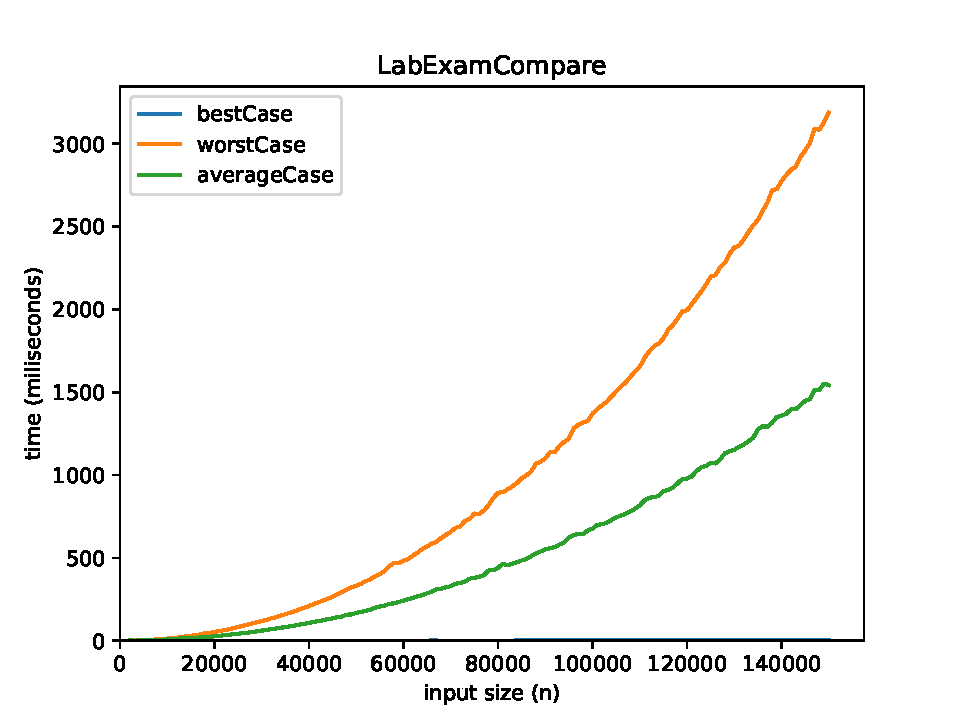
\includegraphics[scale=0.6]{LabExamCompare.pdf}
	\caption{Time (miliseconds) against $n$}
\end{figure}
Clearly, the above graph supports the analysis in (B), as the worst case and best case graphs take the forms we would expect from the theoretical analysis. As the best case grows far slower than the other cases, it is difficult to represent alongside them. Thus figure (2) is included for visual clarity.
\newline
Examining the graph of the average case, we note a parabolic shape. Thus the graph implies that the average case complexity of the algorithm is $\mathcal{O}(n^2)$.
\begin{figure}[H]
	\centering
	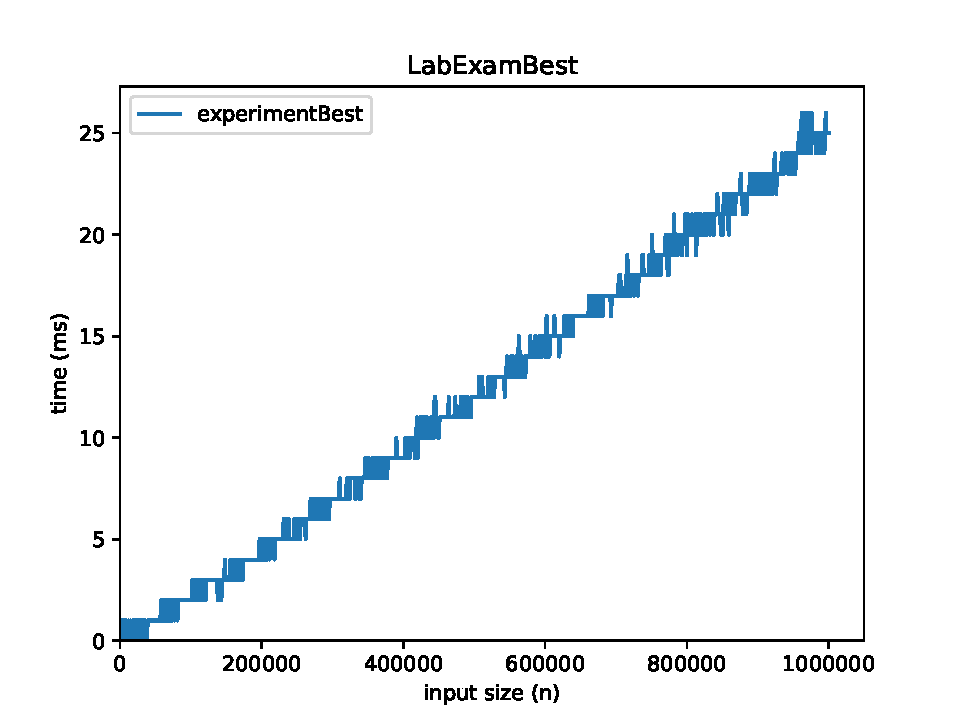
\includegraphics[scale=0.6]{LabExamBest.pdf}
	\caption{Time (miliseconds) against $n$ for the best case, included for clarity. The fluctuations along the linear line are due to the error inherent to such small time scales}
\end{figure}
\newpage
\section{Code}
\lstinputlisting{Program.java}
\end{document} 